\section{The Milestones Project}\label{sec:project}
\epigraph{Direction is more important than speed. We are so busy looking at our 
speedometers \\ that we forget the milestone.}{Anonymous} 

An early overview of the content and aims of the Milestones Project appeared in 
\cite{Friendly:04:gfkl}. 
Here we update that description and provide a few technical details on some 
problems that were encountered in attempting to make the history of data 
visualization convenient for collecting, browsing, searching, and analysis.

\subsection{Origin, structure and evolution}\label{sec:structure}
The initial step in portraying the history of data visualization was to create 
a simple chronological listing of milestone items with capsule descriptions, 
bibliographic references, markers for date, person, place, and links to 
portraits, images, related sources, and more detailed commentaries. 
The initial 
database contained the 105 developments listed by \citet{BenigerRobyn:1978}, 
and incorporated additional records from \citet{Hankins:1999}, 
\citet{Tufte:1983,Tufte:1990,Tufte:1997}, \citet{Heiser:2000}, among others.

This began as a single \LaTeX\ file (with markup tags for all relevant bits of 
information), used to produce a hyper-linked PDF document.  
A variety of 
software tools (perl scripts, Unix utilities) allowed us to turn this single 
source \emph{directly} into the web version originally shown at
\url{http://www.math.yorku.ca/SCS/Gallery/milestone}.  
Other custom software 
tools allowed us to add new milestones items from text files using a template 
of tags (DATE:, AUTHOR:, WHAT:, REF:, IMG:, etc.) and extract the information 
about milestones items, authors, images, etc. in a variety of forms (CSV, XML, 
JSON) that could be used as input for analyses and graphic displays.  
For example, \figref{fig:mileyears4} was produced in SAS software by piping the 
output of a latex to csv translator:
\begin{verbatim} 
itemdb -o milestones.csv < milestones.tex | sas -i milestones.csv mileyears.sas 
\end{verbatim}

It soon became apparent that such a text-based representation was inadequate. 
Updating the milestones data required that the \LaTeX\ file be shared among 
several collaborators; milestone assets, such as images, web links and 
references, were not easily accessible by others, which made collaboration 
cumbersome. 
Further, each update to the web site required an inefficient number 
of steps of verification, re-building, and synchronization with the server, 
meaning the website was often out of date.

Around 2005, we began to make the process into a more dynamic one; to convert 
the flat file into a relational database; create a Milestones administrative 
system and completely redesign the Milestones web site. 
Specifically, we wanted 
to facilitate contributions by any number of trusted collaborators via an 
easy-to-use web administration area, and allow for the dissemination of 
milestones data via an easy-to-browse public user interface.

Migrating the data to this format provided some challenges. 
First, the existing 
milestones data needed to be restructured logically
 and have redundancy minimized. 
To do this, we partitioned the data into its relevant entities: namely the 
milestone itself, and its descriptors, such as its aspect, author, subject, 
keywords, reference, and linked media items (such as images). 
The aspect, 
author, subject, keyword, and reference descriptors exist as a many-to-many 
relationship between it and the milestone. 
For example, an aspect can belong to 
one or more milestones, and the milestone can belong to one or more aspects. 
Media items, on the other hand, can only belong to one milestone at a time, 
with multiple media items possible for a single milestone. 

\figref{fig:datavis-schema-2} illustrates these relationships.  
In this representation, the main table (\texttt{milestone}) contains information regarding each of the items considered a 
milestone in the history of data visualization, linked to other tables (e.g., \texttt{reference}, \texttt{mediaitem}) by unique (primary) keys.  
Other supporting tables (e.g., \texttt{milestone2aspect}) provide for convenient lookups of 
descriptors of these milestones items (\texttt{subject}, \texttt{aspect}, and \texttt{keyword}).

\begin{figure}[!htb]
  \centering
  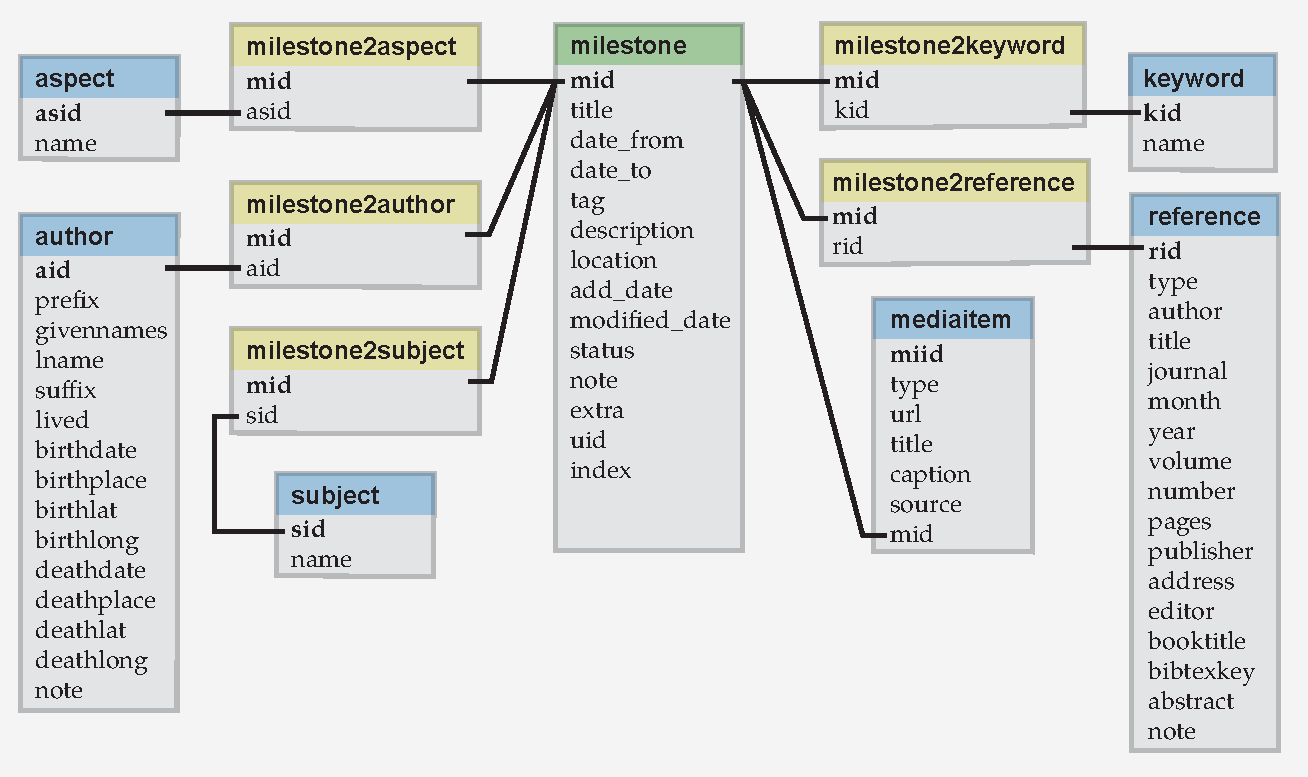
\includegraphics[width=\textwidth,clip]{fig/datavis-schema-3}
  \caption{Simplified schema for the MySQL database for the Milestones Project.}
  \label{fig:datavis-schema-2}
\end{figure}

Normalizing the data in this way enabled us to free the database of 
modification anomalies; ensured that the database structure was scalable, and 
could be extended with minimum modifications. 
Most importantly, it allows for 
future growth, and provides a query-neutral database model \citep{Codd:1971} 
that could be used to power web presentation, and customized indexed search.
The last major benefit, which will be demonstrated in \secref{sec:vistime}, is 
that this schema allows for any type of analysis of the Milestones data itself.

At present, the Milestones Project documents 288 contributions, with nearly 350 
references, information on 336 authors, and 774 media items, made up of 371 
images appearing online on the \url{http://datavis.ca/milestone} site, and 403 
hyperlinks to images and documents that are externally hosted. 
In addition, we 
maintain an offline image database comprising over 1,100 images collected from 
various sources. 
Over time, these too will be incorporated into the database.

\subsection{User interface}
The second challenge related to how to display such a large amount of 
information in an easy-to-use interface that would provide overview, search, 
and details about these events in the history of data visualization. 
We decided 
to retain the time-based grouping of the milestones content by epochs 
(Pre-1600, 1600s, 1700s, etc.), each with a theme (e.g., 1600--1699: 
Measurement and Theory) and descriptive text. 
The visual design of the 
interface adopts Ben Shneiderman's mantra: ``Overview first, zoom and filter, 
then details on demand'' \citep{Shneiderman:1996:IEEE}. 
To do this, we added a 
timeline view (\figref{fig:datavis-timeline2}) of the milestones items 
displayed on the overview landing page.  
In this view, the top panel shows a detailed view of the segment of history highlighted in the bottom panel, 
both of which can be separately scrolled. 
Items in the top panel show a brief text tag, colour-coded by category. 
Clicking on an item in this panel brings up a small description, which is further linked to the details of the milestone item.

\begin{figure}[!htb]
  \centering
  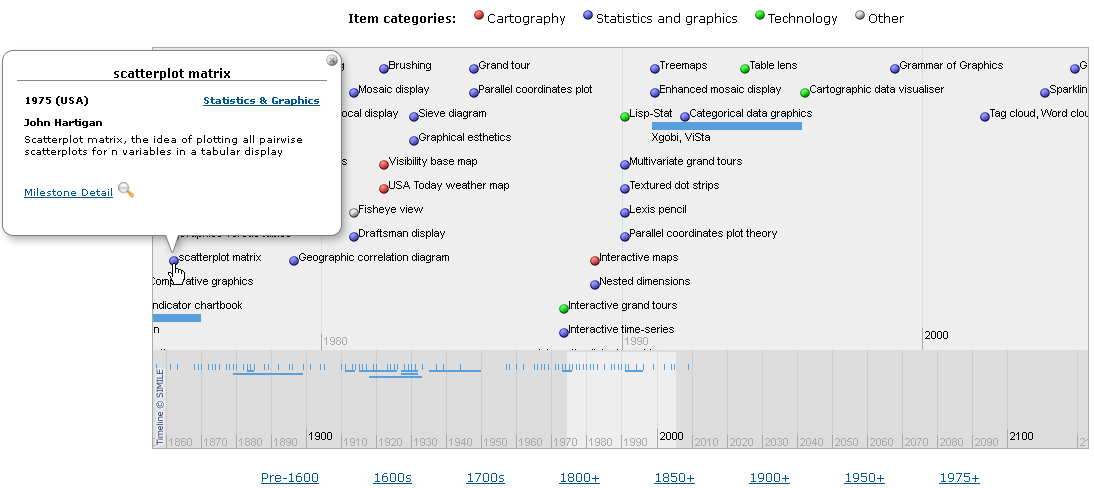
\includegraphics[width=\textwidth,clip]{fig/datavis-timeline2}
  \caption{Timeline view of the Milestones Project from 
  \texttt{http://datavis.ca/milestone}. }  
  \label{fig:datavis-timeline2}
\end{figure}

This timeline, based on the SIMILE Timeline Widget 
(\url{http://www.simile-widgets.org/timeline}), allows multiple connected time 
bands, showing events at different resolutions.  
Each band can be separately 
panned by dragging to the left or right with the mouse pointer, scroll wheel, or 
keyboard arrow keys. 
The timeline view, although most obvious, is just one of 
several possibilities for a visual overview or interaction with the display of 
the milestones database. 
For example, the 
database can also be navigated via a list view (with drop down quick links), 
and in \secref{sec:geography} we will illustrate how it can be explored using a 
map-based display.
The software design of the site, using open-source 
tool kits, makes it relatively simple to add new items, images, etc., since all information
comes from the database.
